% !TEX root = thesis.tex
\graphicspath{ {./figures/} }

%%%%%%%%%%%%%%%%%%%%
\chapter{Evaluation}
%%%%%%%%%%%%%%%%%%%%

% include a discussion on what happens when the delegation graph is invalid, such as when we have a closed loop, or when a node delegates more or less than the entire vote

The three algorithms will be evaluated based on their runtime and scalability as well as their robustness, meaning their ability to handle invalid graphs. 

\section{Runtime and Scalability}

We will explore the runtime of the algorithms on small graphs, big graphs and then explore their behavior in specific situations and corner cases. For the first two sections, we have built an algorithm, that builds a graph with n nodes, and then adds between zero and three delegations per node to random other nodes, ensuring that there are no delegation cycles without a sink. A better explanation of how these graphs are artificially constructed can be found in the Annex. \TODO{Create this annex} We acknowledge, that these assumptions may not be representative of real delegation graphs, where, as studies have shown, delegates tend to not delegate randomly, but to a subset of experts, such as TV personalities, thus centering power to one or few people. This approach also ignores potential tendencies such as friends delegating to eachother more likely. Such situations will be explored in subsection XX. \TODO{Add citations that these situations happen. Maybe the viscous democracy paper, and the pirate party example, and in one of the six original papers Ford shared this was also mentioned}.

\subsection{Small graphs}

\begin{figure}[h]
    \centering
    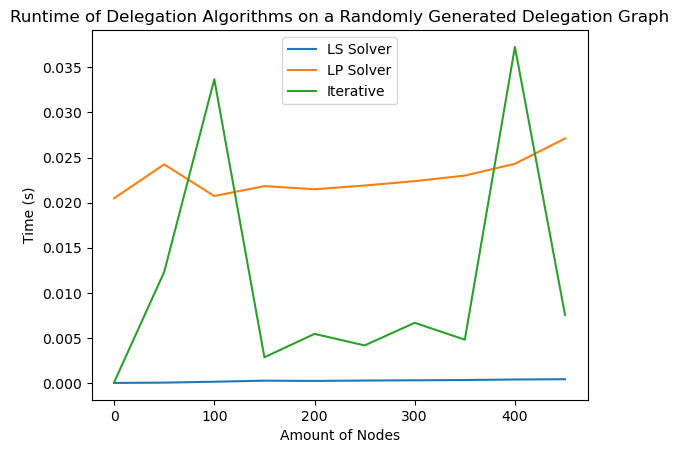
\includegraphics[width=0.4\textwidth]{0-500_random}
    \caption{Runtime of delegation algorithms on a randomly generated delegation graph.}
    \label{fig:random-small}
\end{figure}

In order to explore the three algorithm's behavior on small graphs, we used the graph generator to generate graphs with zero to 450 nodes. After running the set-up each algorithm requires, we timed the runtimes for the algorithms to resolve the delegations. Since the runtimes are very small, we timed the runtime for 100 iterations of each algorithm, in order to exclude as best as possible any fluctuations in runtime caused by background processes or measurement fluctuations, divided this runtime by the amount of iterations to find an average runtime value. Figure \ref{fig:random-small} shows the results of this benchmark.

We can see, that the LS Implementation, optimized for sparse matrices, outperforms the other two algorithms. Its growth in runtime is so small, that the line looks to be staying flat on the x-axis. However, with a graph of 450 nodes, its runtime is about 0.0004 seconds. Both the LS and LP implementation display a rather steady, yet growing runtime. The LP solver seems to have some overhead, since even when the graph has zero nodes, it has a runtime of about 0.02 seconds.

Furthermore, we can interestingly observe large spikes in the runtime of the iterative approach. Exploring this more closely, we find that, using a seed of 100, the graph with 11 nodes takes the iterative algorithm a lot more time than the graph with 10 or 12 nodes, as shown in Figure \ref{fig:random-tiny}. At 10 nodes, the runtime of the iterative algorithm is just about 0.004 seconds, at 12 nodes it is 0.001 seconds, so even slightly faster than the slightly smaller graph, but when the graph has 11 nodes, the runtime skyrockets to about 0.067 seconds.

\begin{figure}[h]
    \centering
    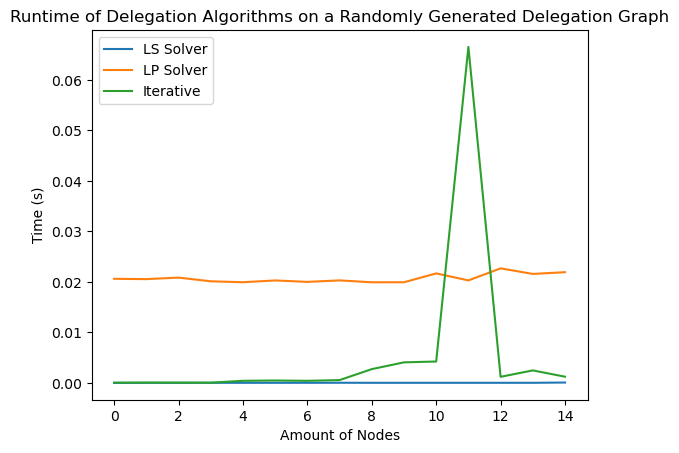
\includegraphics[width=0.4\textwidth]{0-15_random}
    \caption{Runtime of delegation algorithms on a randomly generated delegation graph.}
    \label{fig:random-tiny}
\end{figure}

A possible explanation for this spike may be, that when the graph has 10 and 12 nodes, it iterates only 643 and 149 times respectively, before cutting off, while when it has 11 nodes it iterates 8064 times before cutting off. Figure \ref{fig:random-11and12} shows the two graphs with 11 and 12 nodes.

\begin{figure}[h]
    \centering
    \begin{subfigure}[t]{0.45\textwidth}
        \centering
        \fbox{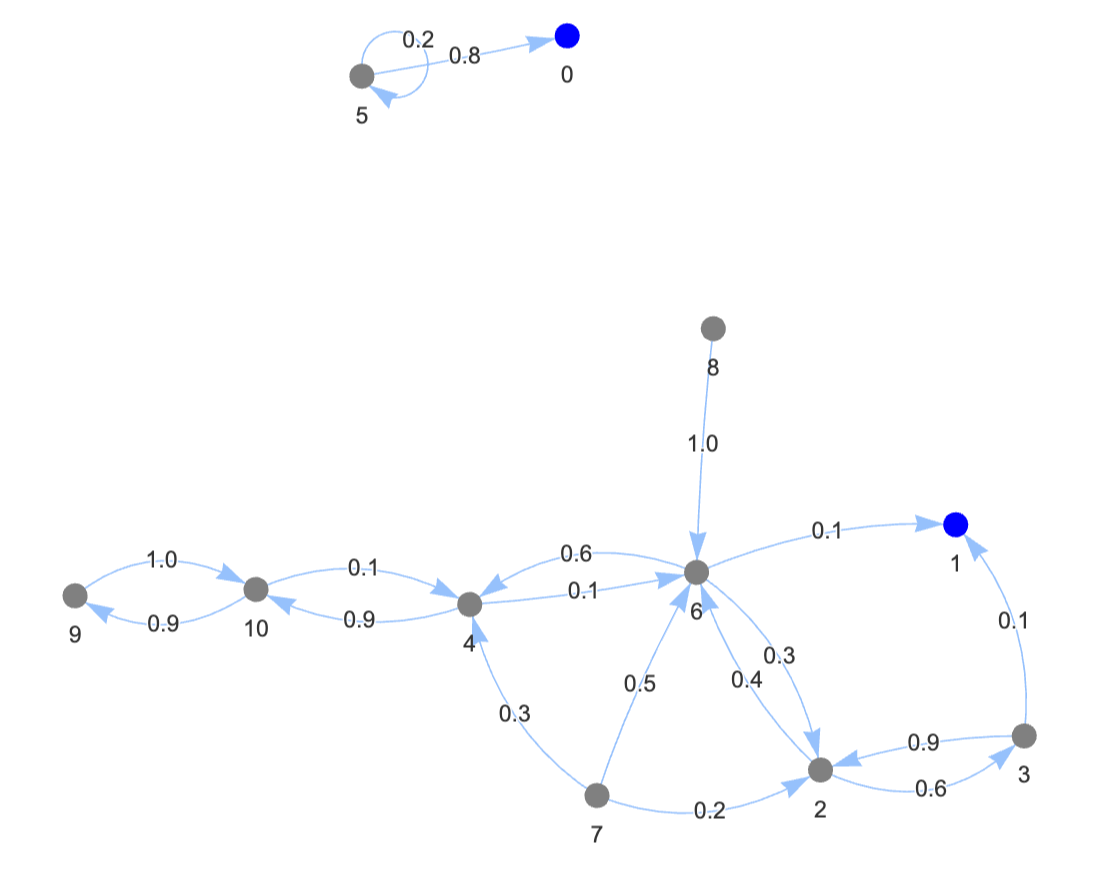
\includegraphics[width=\textwidth]{11_random}}
        \caption{11 nodes}
    \end{subfigure}
    \hfill
    \begin{subfigure}[t]{0.45\textwidth}
        \centering
        \fbox{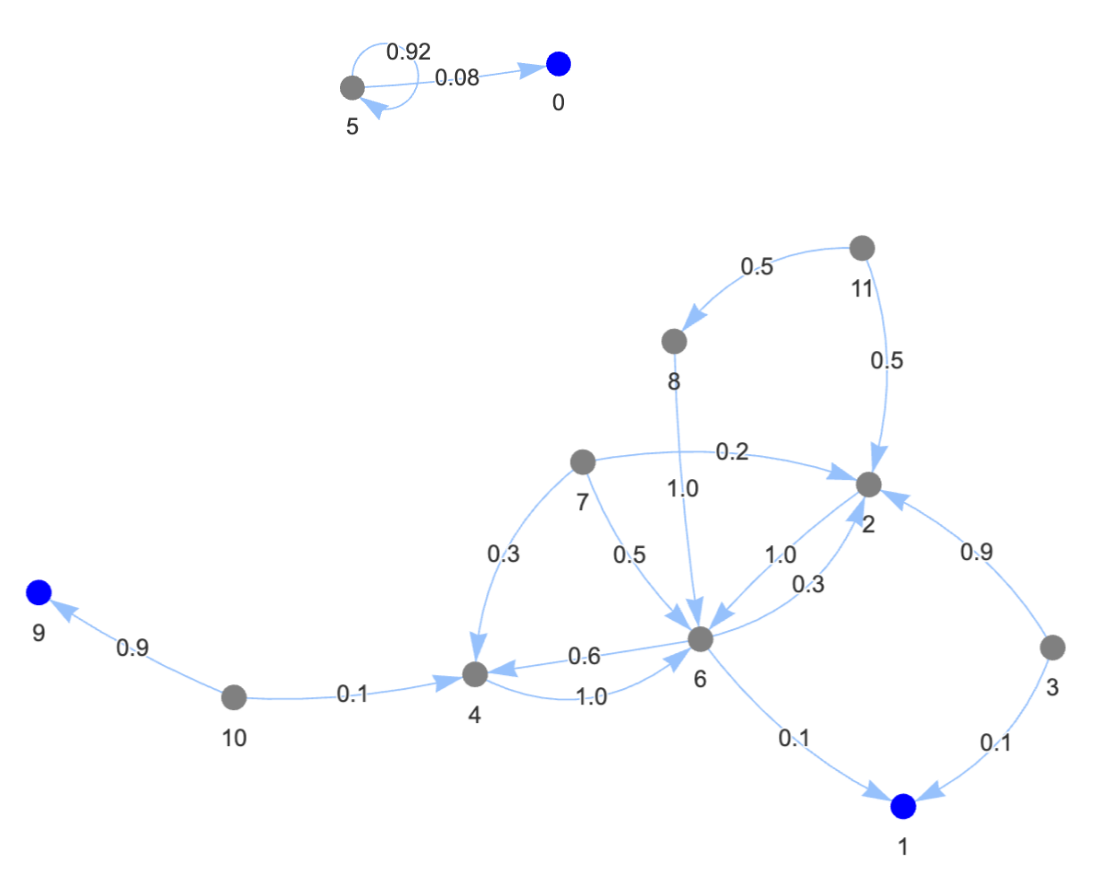
\includegraphics[width=\textwidth]{12_random}}
        \caption{12 nodes}
    \end{subfigure}
    \caption{Delegation graphs with 11 and 12 nodes}
    \label{fig:random-11and12}
\end{figure}

Inspecting them reveals a possible explanation for this behavior. When the graph has 12 nodes, node \texttt{9} is a sink, while it delegates its power back to node \texttt{10} when the graph has only 11 nodes. In the latter case, power going out of node \texttt{9} needs to pass to node \texttt{10}, \texttt{4} and \texttt{6} before reaching a node. While passing through node \texttt{4}, we can see that 90\% of the power is delegated back into the cycle between nodes \texttt{4}, \texttt{10} and \texttt{9}. The algorithm will iterate power through this loop, until enough has been drained out for the \texttt{max\_change} to fall below the cutoff. 

This is an important shortcoming of the iterative algorithm. Power can easily get trapped within permissible cycles that only have a small drain allowing the power to escape from the cycle. Each iteration, if a great proportion of the nodes with draining edges' power is sent back into a cycle, the algorithm needs to continuously iterate until the power is back at the drain nodes, however depending on the cycle this may happen very inefficiently. This phenomenon will be tested more in section \ref{subsec:cycles_draining}

\subsection{Large Graphs}

Delegation graphs may grow arbitrarily large. National elections for example can contains up to hundreds of millions of participants. Thus we will explore how the algorithms perform when having to resolve graphs with a lot of nodes. Again, the graphs will be randomly generated, such that each nodes has between 0 and 3 delegates. 

\begin{figure}[h]
    \centering
    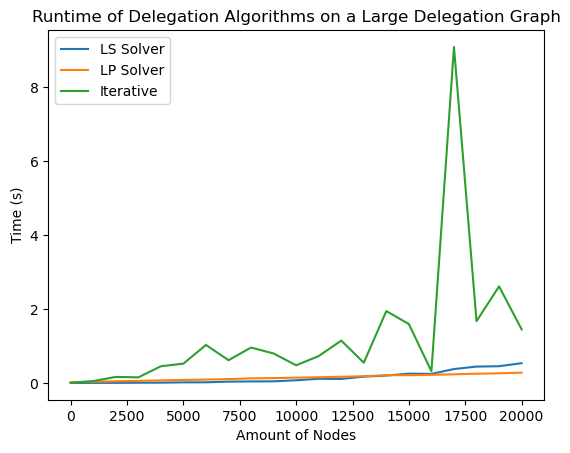
\includegraphics[width=0.4\textwidth]{0-20000_random}
    \caption{Runtime of delegation algorithms on a randomly generated delegation graph.}
    \label{fig:random-large}
\end{figure}

In figure \ref{fig:random-large} we can see, that it is difficult to determine a pattern in the runtime for the iterative algorithm. Depending on the underlying delegation graph, the runtime can grow unpredictably large. What is evident from the runtime graph however, is that in as the graphs get larger its runtime never subceeds the runtimes of the other two algorithms, while it is worth mentioning that for some graphs, the iterative algorithm's runtime is not a lot longer than that of the other two algorithms. It is difficult to make any statement about the runtime class of the iterative algorithm based just on the number of nodes in the graph, since, depending on the structure of the graph and the cutoff value the runtime can get arbitrarily high. The comparatively high runtime of the iterative algorithm overshadows the runtimes of the other two, so in order to better discuss and analyze their performance, figure \ref{fig:random-large-no-iterative} shows the same graph as in figure \ref{fig:random-large}, without the runtimes for the iterative algorithm.

\begin{figure}[h]
    \centering
    \begin{subfigure}[t]{0.45\textwidth}
        \centering
        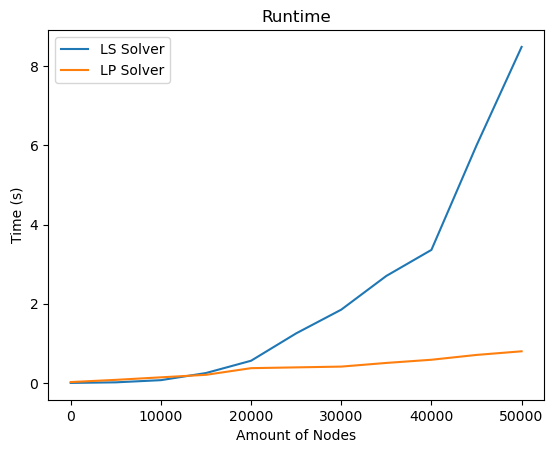
\includegraphics[width=\textwidth]{0-50000_random_no_iterative}
        \caption{Linear scale}
         \label{subfig:random-large-no-iterative-linear}
    \end{subfigure}
    \hfill
    \begin{subfigure}[t]{0.45\textwidth}
        \centering
        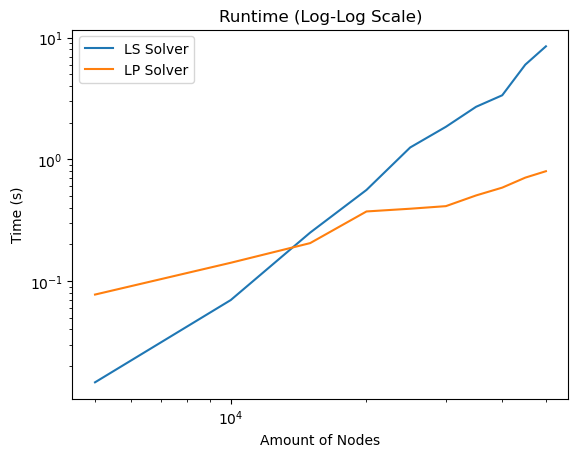
\includegraphics[width=\textwidth]{0-50000_random_no_iterative_loglog}
        \caption{Loglog scale}
         \label{subfig:random-large-no-iterative-loglog}
    \end{subfigure}
    \caption{Runtime of delegation algorithms on a randomly generated delegation graph.}
    \label{fig:random-large-no-iterative}
\end{figure}

\begin{figure}[h]
    \centering
    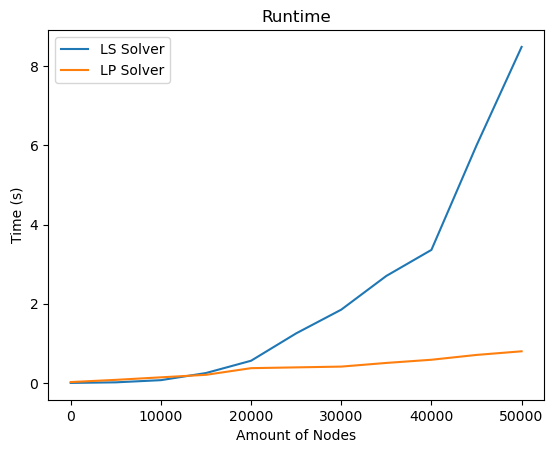
\includegraphics[width=0.4\textwidth]{0-50000_random_no_iterative}
    \caption{Runtime of delegation algorithms on a randomly generated delegation graph.}
    \label{fig:random-large-no-iterative}
\end{figure}

% maybe have a look at the log-log graph to show whether or not its a power law

Figure \ref{subfig:random-large-no-iterative-linear} shows, that as the delegation graph grows, the LP solver's runtime grows more slowly than the LS Solver's. For resolving smaller graphs, the LS solver outperforms the LP solver, with a runtime of almost zero for empty or very small graphs, while the LP solver has a clearly non-zero runtime even for very small graphs. However, at around 12 000 nodes, this changes, as the LP solver's runtime's slower growth catches up with that of the LS solver. 

The type of growth, so the runtime class, is not immediately clear from the graphs, although the LP solver's growth seems to be more linear than that of the LS solver. Looking at the same results on a loglog graph reveals, that the LS solvers runtime may follow a power law.

Fitting the data into different kinds of curves reveals, that the LP implementations runtime likely has linear growth, while the LS solver grows following a power distribution, such that it is in the runtime class of $O(n^{2.778})$.

\TODO{I should either put the runtime results and/ or the code and the regression results into the annex, or into the text...}

\subsection{Dense Graphs}

While we expect most delegators in any delegation graph to only delegate to a handful of people, a well formed delegation graph can have any number of delegates per delegator. Thus, it may also be interesting to compare how the three algorithms compare when resolving denser graphs. In this section, test the three implementations on complete graphs, which have been adapted to be well formed delegation graphs. In a complete graph, all nodes are connected to all other nodes. Thus, in order to be well-formed delegation graphs, we remove outgoing edges of nodes, turning them into sinks, until 10\% of the nodes are sinks. Then, each delegators vote is equally distributed to all of its outgoing edges, such that the edge weights add up to 1. Finally, any closed delegation cycles are removed by removing a random edge in the cycle (and re-normalizing the edge weights). 

\TODO{Make this entire paper use "closed delegation cycles", and define them properly if that hasn't happened yet.}


\subsection{Cycles with Weak Draining Edges}
\label{subsec:cycles_draining}

\section{Robustness}

%Here, mention that cycles can be easily broken by like one little delegation outward